%! Author = mboehme
%! Date = 20.03.2023

\section{Anhang}\label{sec:anhang}
\newline
\newline
\subsection{Objektorientertes Design}\label{subsec:objektorientiertes-design}
\newline
\newline
\par\vspace{1cm}
\centering
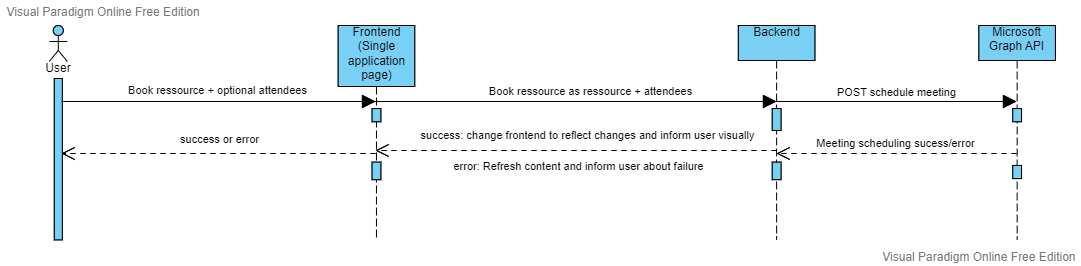
\includegraphics[width=0.5\textwidth]{Bilder/Objektorientiertes Design/Sequence diagram for ressource booking (3)}
\caption{Sequenzdiagramm für die Anwendung}
\label{fig:sequence-diagramm}
\newline
\newline
\par\vspace{1cm}
\centering
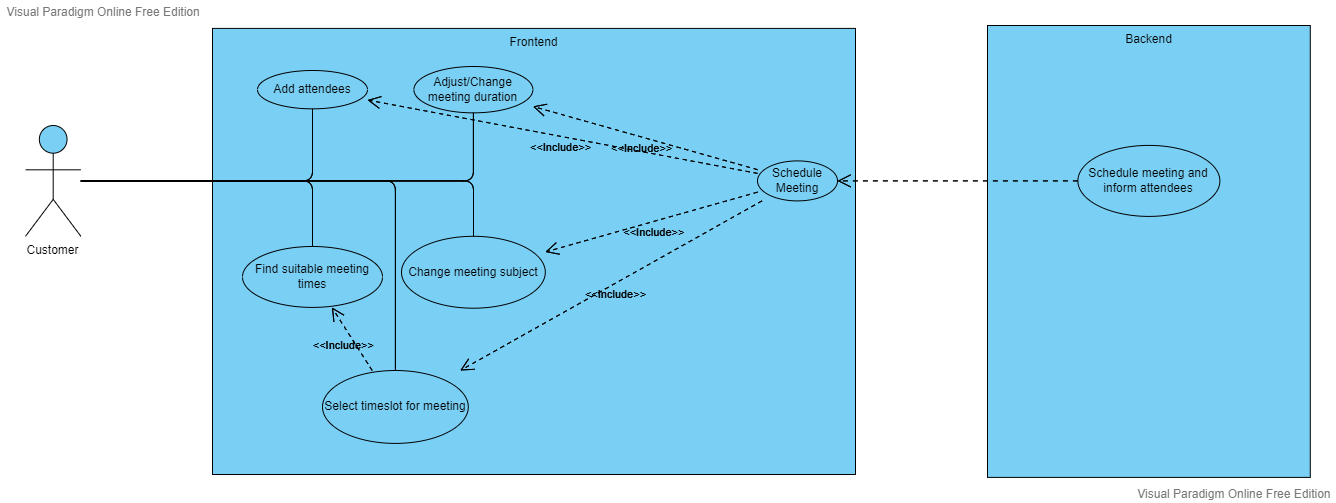
\includegraphics[width=0.5\textwidth]{Bilder/Objektorientiertes Design/Use Case diagram ressource booking}
\caption{Use-Case-Diagramm für die Anwendung}
\label{fig:use-case-diagramm}
\newline
\newline
\newpage
\subsection{Objektorientierte Analyse}\label{subsec:objektorientierte-analyse}
\par\vspace{1cm}
\centering
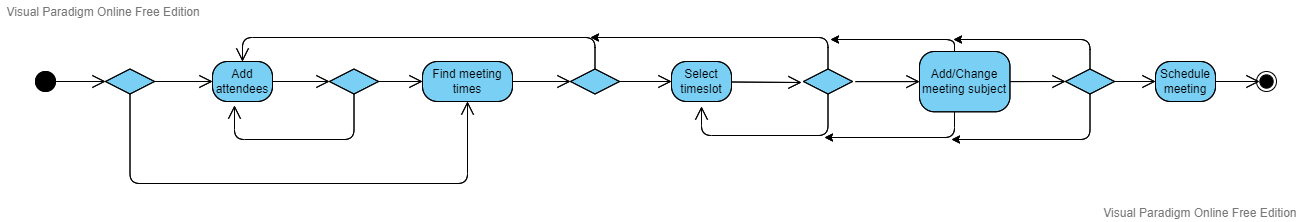
\includegraphics[width=0.5\textwidth]{Bilder/Objektorientierte Analyse/Ressource booking activity diagramm}
\caption{Aktivitätsdiagramm für die Anwendung}
\label{fig:aktivitaetsdiagramm}
\newline
\newline
\par\vspace{1cm}
\centering
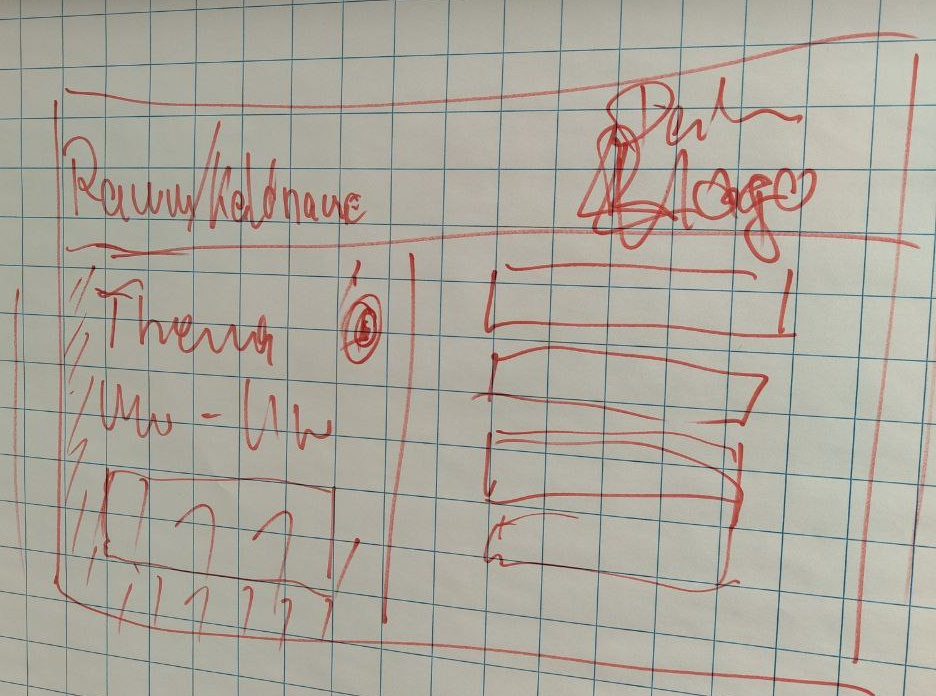
\includegraphics[width=0.5\textwidth]{Bilder/Raumanzeige_grob.jpeg}
\caption{Raumanzeige Mockup vom ersten Meeting}
\label{fig:raumanzeige-mockup}
\newline
\newline
\newpage

\par\vspace{1cm}
\centering
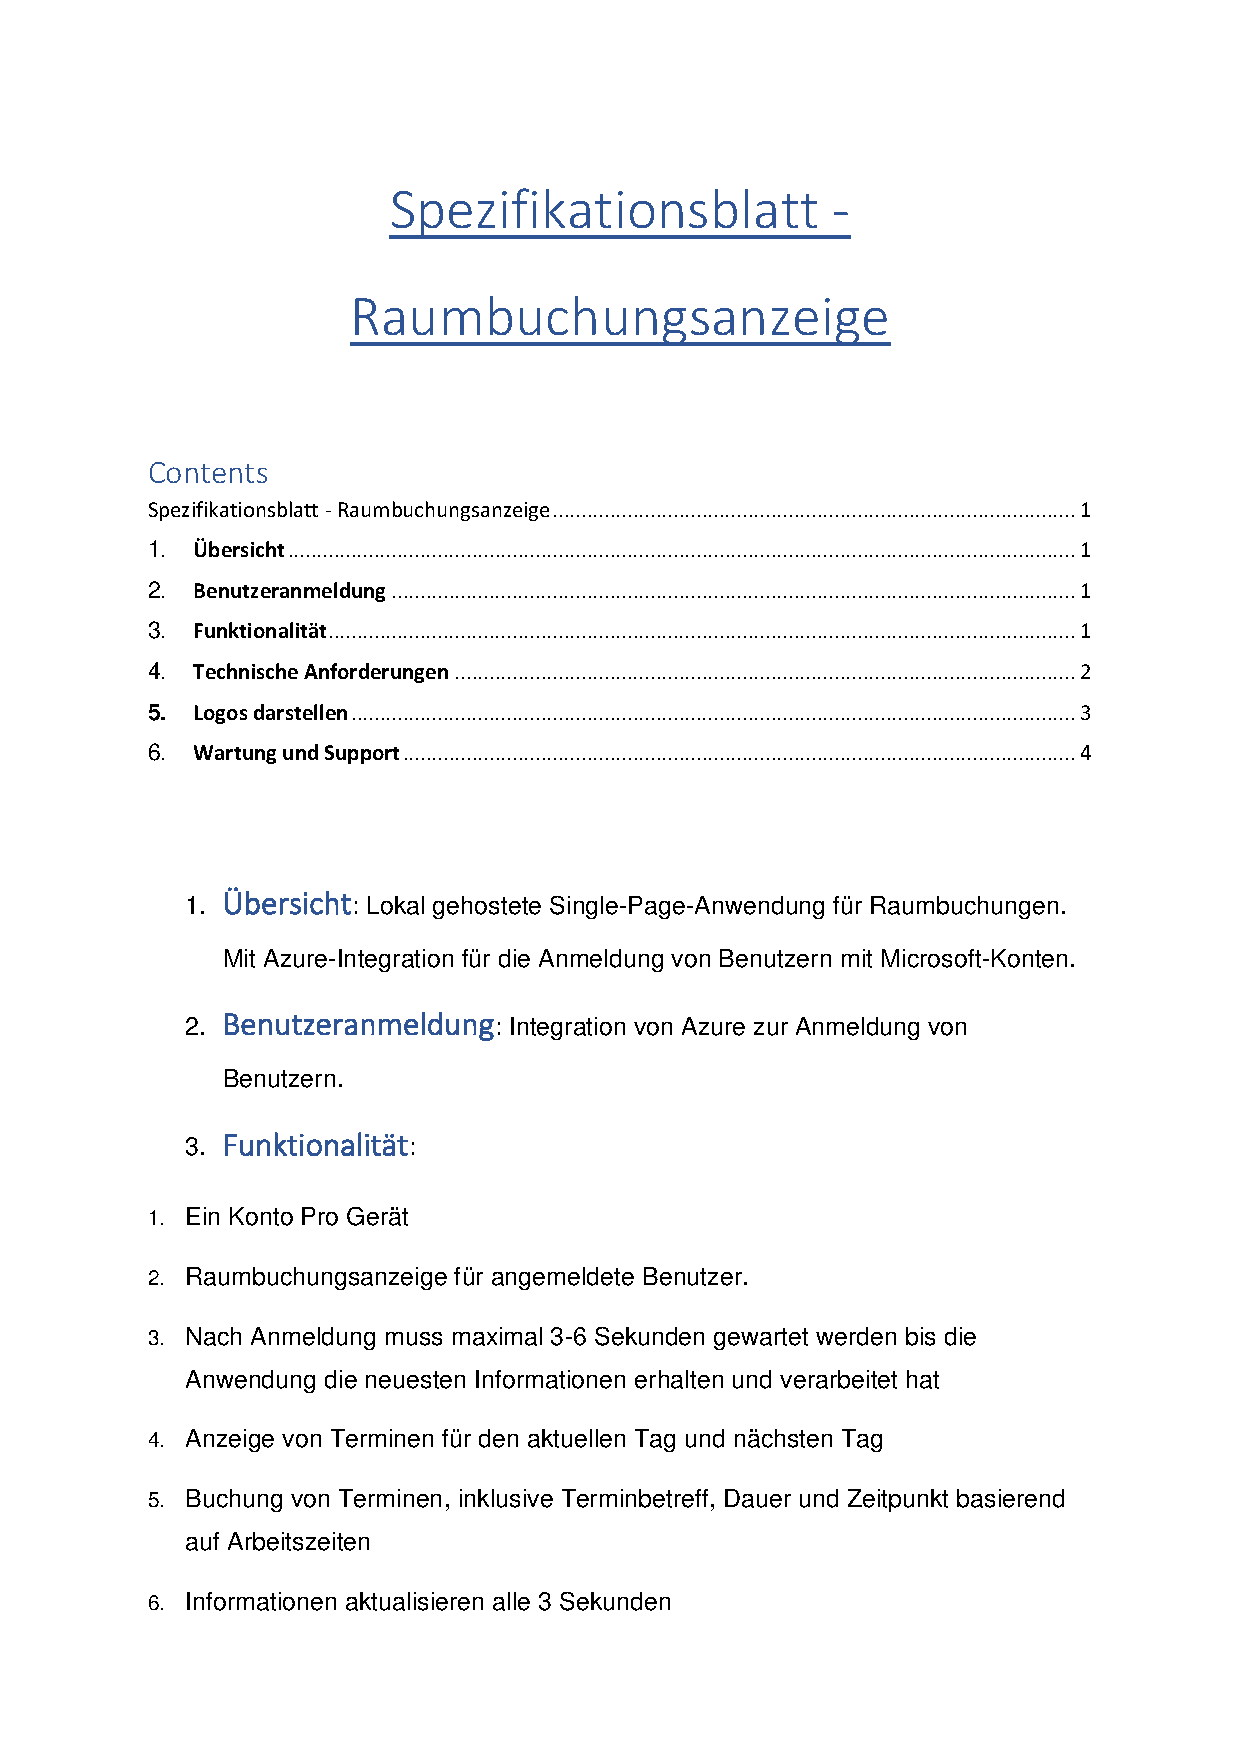
\includepdf[pages=1,pagecommand={},scale=0.8,pagecommand={\subsection{Spezifikationsblatt}\label{subsec:spezifikationsblatt}}, width=\textwidth]{PDFs/Spezifikationsblatt - Raumbuchungsanzeige - Office365 room booking - censored details.pdf}
\includepdf[pages={2-}, scale=0.8]{PDFs/Spezifikationsblatt - Raumbuchungsanzeige - Office365 room booking - censored details.pdf}
\caption{Spezifikationsblatt für die Anwendung}
\label{fig:spezifikationsblatt}
\newline
\newline